%%%%%%%%%%%%%%%%%%%%%%%%%%%%%%%%%%%%%%%%%%%%%%%%%%%%%%%%%%%%%%%%%%%%%%%%%%%%%
\chapter{Umsetzung}
\label{chap:Umsetzung}
%%%%%%%%%%%%%%%%%%%%%%%%%%%%%%%%%%%%%%%%%%%%%%%%%%%%%%%%%%%%%%%%%%%%%%%%%%%%%

\section{Technologien}
\subsection{Java}
Die drei Teilprojekte der Arbeit wurden in Java entwickelt. Die verwendete Java Version ist Java 11. Java wird als plattformunabhängige und robuste Programmiersprache verwendet. Auch in der Entwicklung der mobilen Applikation wird Java eingesetzt. Als Alternative zu Java könnte C-Sharp oder eine JavaScript basierende Webserver-Lösung wie Node.js fungieren.
\subsection{Android}
Die mobile Applikation ist eine Android-Anwendung. Als Programmiersprache wurde Java verwendet. Eine gute Alternative zu Java bietet Kotlin, da der Code kompakter und einfacher zu schreiben ist ~\parencite{banerjee2018comparative}. Aus Gründen der Einfachheit und Lesbarkeit wurde aber die Programmiersprache Java für die Entwicklung in Android gewählt. Ebenso bietet Android NDK (Native Development Kit) eine Alternative, mit der die mobile Applikation in C oder C++ entwickelt wird. Mit Android NDK kann schneller und wiederverwendbarer Code geschrieben werden, da der Code auch für andere Plattformen verwendet werden kann ~\parencite{ratabouil2015android}. Die Applikation wurde sowohl mit einem virtuellen Android-Emulator, als auch mit einem Android-Device getestet.
\subsection{Spring}
Spring, bzw. Spring Boot ist ein Java Framework, das im Zuge der Projektarbeit zur Entwicklungder Web-Applikation verwendet wurde. Spring Boot bietet zusätzlich unter anderem einen eingebetteten Server,  mit dem die Applikation schnell und einfach gestartet werden kann. Auch die Userverwaltung und damit auch die Security-Aspekte wurden mit Spring (Spring Security) entwickelt. Als mögliche Alternative zu Spring mit Spring Security kann Java EE mit einem OAuth2 eingesetzt werden. \ref{pressmarSpring}
\subsection{Maven und Gradle}
Maven ist ein Versionsverwaltungstool mit dem Abhängigkeiten und JARs verwaltetund heruntergeladen werden können. Maven wird hierbei in der Webapplikation und im Plugin eingesetzt. Eine Alternative zu Maven ist das Tool Gradle, welches in der Android Applikation für das Build-Management eingesetzt wurde.
\subsection{Thymeleaf}
Tyhmeleaf ist eine Template-Engine, die in HTML eingesetzt werden kann. Eine Template-Engine nimmt ein vorgefertigtes HTML-Skript (Template) und initialisiert dynamische Werte in die angegebenen Platzhalter. Thymeleaf gehört zu den Server-Side-Engines, das heißt die angezeigte Seite wird am Server generiert ~\parencite{searchmetrics}. Thymeleaf wird in der Webapplikation verwendet, um die Userverwaltung in der Weboberfläche zu implementieren. Der Vorteil dabei ist, da so eine einfache Interaktion mit dem Server stattfinden kann. Diese Interaktion ist beispielsweise die Anmeldung, bei der das angegebene Passwort validiert, überprüft und eine Validierungsnachricht zurückgegeben wird. Als Alternative kann JSF eingesetzt werden. 
\subsection{MongoDB}
Als Datenbank wird die nicht-relationale Lösung MongoDB verwendet, da es verschie-dene Vorteile gegenüber relationales Datenbankmanagementsystem bietet (siehe Punkt4.4.1). Es gehört zu den dokumentorientierten Datenbanken. MongoDB kann über die offiziele Website heruntergeladen und installiert werden. \footnote{https://www.mongodb.com/try/download/community}
\subsection{MongoDB Java Driver}
Der MongoDB Java Driver wird für die Kommunikation (Synchronisation und asyn-chrone Interaktion) mit MongoDB eingesetzt. Mit dem Driver werden unter anderem erstellten Benutzer in die Datenbank gespeichert und ausgelesen.
\subsection{IntelliJ und Android Studio}
Als Entwicklungsumgebungen wurden IntelliJ und Android Studio gewählt, da diese IDEs mehrere verschiedene Sprachen unterstützen und Android Studio eine Abwandlung von IntelliJ ist und daher die Entwicklung sehr einfach und nur minimal unterschiedlich ist.
\subsection{Git und SourceTree}
Git wurde für die Versionsverwaltung verwendet. Ebenso wird in der Applikation mit Git über eine GithubAPI kommuniziert und Daten abgefragt. \footnote{https://developer.github.com/v3/} (siehe Punkt 3.2.1 Konzept: Webapplikation). Statt Git kann auch die Software SVN(Apache Subversion) eingesetzt werden, welches aber verschiedene Nachteile hat wie ein schweres Branch-Handling. Als Git-basiertes Versionsverwaltung-Managementtool wird SourceTree verwendet.
\subsection{HTML, JavaScript und CSS}
Die Weboberfläche wurde mit diesen Technologien entwickelt. Ebenso wurden verschiedene JavaScript-Plugins und das CSS/JS-Framework Bootstrap verwendet, mit dem schnell und einfach Weboberfläche gestaltet werden können. Als Alternative zu HTML dienen Frameworks wie JavaEE Technologie JSF (Java Server Faces).
\section{Userverwaltung}
\subsection{Vorteile der Userverwaltung}
Ein Usermanagement mit Sicherheitsimplementierungen ist ein integraler und wichtiger Teil einer Webapplikation, in der sensible Daten behandelt werden, ebenso eignet sich in den gegebenen Anwendungsfällen eine Benutzerverwaltung besonders. Die Userwaltung ergibt daher folgende Vorteile:
\begin{itemize} 
  \item \textbf{Unterstützung für den Benutzer/die Benutzerin} 
Mit der Unterstützung der Userverwaltung können genauere Informationen und Berichte für den angemeldeten Benutzer angezeigt werden. Voraussetzung dafür ist aber die Integration und Verwendung eines Versionsverwaltungs-Management-Tools. So können die Fehler und Probleme der erstellten Files den Entwickler oder der Entwicklerin zugeordnet werden, welcher auf der Weboberfläche eingesehen werden können. So kann der User seine Fehler überblicken und gezielt ausbessern. Durch diese Individualisierung kann auch eine mögliche Verbesserung der Entwicklungsfähigkeit eintreten.  
    \item \textbf{Sicherheit und Zugriffsschutz} \\ Ein anderer wichtiger Punkt ist der Security-Aspekt. Die Webapplikation kann sowohl in einem Unternehmen, oder privat auf einem eigenen Server installiert werden. In beiden Fällen ist ein Zugriffsschutz notwendig, um unberechtigten Benutzer den Zugriff zu verweigern und sensible Daten zu schützen. Die Daten, die in der Webapplikation angezeigt werden müssen sehr vertraulich behandelt werden, da in der Weboberfläche neben weniger wichtigen Code-Smells auch zum Beispiel Sicherheitsprobleme angezeigt werden können. Diese Sicherheitsprobleme können von Angreifern ausgenutzt werden. Auch wenn die Applikation in einem gesicherten Firmennetzwerk installiert wird, ist die Implementierung eines Zugriffsschutzes wichtig. 
\item \textbf{Unterstützung für das Team}
Eigene Entwicklungsteams werden mithilfe einer Benutzerverwaltung erstellt. Dazu können zu den einzelnen Projekten Entwicklerinnen, Entwickler und andere am Projekt beteiligten Personen (Scrum-Master, Tester, usw.) hinzugefügt werden. Nur Mitglieder in diesen Teams können so die Fehler und Bugs einsehen. Den Usern werden daher nur die Projekte angezeigt, an welchen sie auch beteiligt sind. Außerdem können mithilfe der User- und Teamverwaltung eigene und spezielle Reports erstellt werden.
\end{itemize}

\subsection{Allgemeiner Aufbau} 
\textbf{User Flow}
Die Benutzerin oder der Benutzer sehen beim Aufrufen der Website, automatisch den Login. Ohne einer richtigen Anmeldung, kann man nicht auf die API oder die Webanwendung zugreifen. Der Benutzerin, der Benutzer muss sich vorher mit einer Email-Adresse und einem Passwort registrieren. Wenn eine Abmeldung nicht manuell erfolgt, so wird der User automatisch abgemeldet.
\textbf{Berechtigung zur Datenanzeige}
Um auf Projekt-Inhalte zugreifen zu können, muss ein Projektmitglied die Email-Adresse des neuen Teammitglieds zum Projekt hinzufügen. Erst wenn die Email-Adresse für das Projekt hinterlegt ist, werden die Fehler und Bugs des Projekts angezeigt. Eine andere Möglichkeit dieses Sicherheitsmechanismus wäre eine Anfrage der Entwicklerin oder des Entwicklers an das Team, welches dann die Email-Adresse akzeptieren oder ablehnen kann. So können keine unberechtigten Personen auf sensible Daten zugreifen. Eine Hierarchie-Regelung bzw. verschiedene Berechtigungsstufen sind nicht implementiert, da das Projektteam als Scrum-Team angesehen wird und im Scrum-Prozess alle Mitglieder gleichberechtigt sind \ref{scrumprozess}. Jedes Teammitglied kann daher ein neues Teammitglied mit der Email-Adresse hinzufügen.
\textbf{Administrator und initialer Zugriff}
Werden mit dem Datenbank-Importer-Plugin die Ergebnisse der Statischen Code Analyse eines bestimmten Projekts zum ersten Mal in die Datenbank geladen, so wird eine initiale Projektkonfiguration angelegt. Als erstes Mitglied wird automatisch ein Administrator gewählt. Dieser Administrator kann dann die ersten Teammitglieder, zum Beispiel die Projektleiterin oder den Projektleiter, in das Team einladen. So wurde das Problem gelöst, dass User zu Projekten nur eingeladen, aber nicht beitreten können. Ohne diese Implementierung kann aber kein User einen anderen User einladen, da zuerst kein User Mitglied des Teams ist. Die Mail-Adresse dieses Administrators muss im Plugin angegeben werden. Bei wiederholten Importen aus dem gleichen Projekt in die Datenbank, wird keine neue Konfiguration mehr erstellt.

\subsection{Implementierung des Usermanagements mit Spring Security}
\subsubsection{Allgemein}
Die Benutzerinnen und Benutzer werden in der Datenbank gespeichert. In der Datenbank wird dazu eine eigene Collection für die User angelegt. Die Passwörter werden verschlüsselt. In der Weboberfläche werden die Daten in einer Thymeleaf-UI eingegeben. Dazu müssen die Dependencies \textit{thymeleaf-layout-dialect} und \textit{spring-boot-starter-security} eingebunden werden. 
\subsubsection{Security Service}   
Im Security Service werden die Userdaten ausgelesen und gespeichert. Das Service implementiert die Spring-Security Schnittstelle \textit{UserDetailsService}. Beim Speichern wird das Passwort des an die Methode übergebenen Users überschrieben (siehe \ref{lst:phase}). Der \textit{BCryptPasswordEncoder} wird hierbei von Spring definiert und verschlüsselt das Passwort als Hash \footnote{https://docs.spring.io/spring-security/site/docs/4.2.15.RELEASE/apidocs/org/springframework/security/crypto/bcrypt/BCryptPasswordEncoder.html}. 

\lstset{
  caption={Speichern und Auslesen des Users. Beim Speichern des Benutzers wird das Passwort automatisch verschlüsselt.}, 
  basicstyle=\small\ttfamily, 
  label=lst:phase, 
  %float=tbhp, % float image to top/bottom/here/page
  language=Java,
  frame=single,
  breaklines=true, % break long source code lines, and add arrow
  postbreak=\mbox{\textcolor{red}{$\hookrightarrow$}\space},
  %  basewidth={0.55em}, 
  % fontadjust}  % adjust these for more appealing appearance
}

% listing with some settings, such as float, for this listing only
\begin{samepage}% with samepage we keep a FLOATing listing on one page
	\begin{lstlisting}[float=tbhp]
@Autowired
private BCryptPasswordEncoder passwordEncoder;

public void saveUser(User user) {
    user.setPassword(
       passwordEncoder.encode(user.getPassword()));
    mpngoUserService.saveUser(user);
}

@Override
public UserDetails loadUserByUsername(String email) 
  throws UsernameNotFoundException {

    User user = passwordEncoder.findByEmail(email);
    if (user != null) {
      List<GrantedAuthority> authorities =     
        getUserAuthority(user.getRoles());
          return authenticateUser(user, authorities);
    } else {
          throw new UsernameNotFoundException
             ("username not found");
    }
}
	\end{lstlisting}
\end{samepage}
Die Passwort-Überprüfung und der Aufruf der Methode \textit{loadUserByUsername} wird hierbei von Spring selbst implementiert.  Dazu muss das Datenbank-Objekt \textit{User} zum Spring-Objekt \textit{UserDetails} gemappt und eine eigene Configuration-Klassen implementiert werden (siehe Listing \ref{lst:config}). Im Security-Service sind ebenso Berechtigungsüberprüfungen implementiert. Dazu müssen Rollen erstellt und den Benutzer zugewiesen werden. Diese Rollen bzw. Berechtigungen werden mithilfe der \textit{GrantedAuthority} gespeichert und ausgelesen.

\lstset{
  caption=[Konfiguration für das Spring Security UserService]{Konfiguration für das Spring Security UserService. Das Service \textit{UserSecurityService} wird nun als das zentrale Service für die Useroperationen von Spring Security verwendet.}, 
  basicstyle=\small\ttfamily, 
  label=lst:config, 
  %float=tbhp, % float image to top/bottom/here/page
  language=Java,
  frame=single,
  breaklines=true, % break long source code lines, and add arrow
  postbreak=\mbox{\textcolor{red}{$\hookrightarrow$}\space},
  %  basewidth={0.55em}, 
  % fontadjust}  % adjust these for more appealing appearance
}

% listing with some settings, such as float, for this listing only
\begin{samepage}% with samepage we keep a FLOATing listing on one page
	\begin{lstlisting}[float=tbhp]
@Bean
public UserDetailsService userDetailService() {
    return new UserSecurityService();
}

@Override
protected void configure
   (AuthenticationManagerBuilder auth) throws Exception {
     UserDetailsService detailsService = userDetailService();
     auth.userDetailsService(detailsService)
        .passwordEncoder(bCryptPasswordEncoder);
}
	\end{lstlisting}
\end{samepage}
Werden hier andere Datenbanken oder Services implementiert, so muss nur die Implementation für das Repository bzw. in diesem Fall das \textit{mpngoUserService} ausgetauscht werden. 
\subsubsection{Security Konfigurationen}
Um die Applikation (URLs der einzelnen Unterseiten) und die API schützen zu können, müssen nun weitere Konfigurationen hinzugefügt werden ~\parencite{springSecBook}. Dazu müssen die einzelnen URLs für die Anzeige der Daten gesichert werden, während hingegen die URLs für den Login und den Website-Aufruf frei zugänglich sein müssen. Auch die Logout-URL kann hier angegeben werden \ref{lst:configurls}.
\lstset{
  caption=[Konfiguration für die Sicherheit der URLs.]{Konfiguration für die Sicherheit der URLs. Die einzelnen Paths können entweder für alle freigegeben oder für eine bestimmte Gruppe angezeigt werden. Das Abmelden wird von Spring automatisch durchgeführt.}, 
  basicstyle=\small\ttfamily, 
  label=lst:configurls, 
  %float=tbhp, % float image to top/bottom/here/page
  language=Java,
  frame=single,
  breaklines=true, % break long source code lines, and add arrow
  postbreak=\mbox{\textcolor{red}{$\hookrightarrow$}\space},
  %  basewidth={0.55em}, 
  % fontadjust}  % adjust these for more appealing appearance
}

% listing with some settings, such as float, for this listing only
\begin{samepage}% with samepage we keep a FLOATing listing on one page
	\begin{lstlisting}[float=tbhp]
...
http.antMatchers("/login").permitAll()
.antMatchers("/reports").hasAuthority("USER")
.and().logout()
.logoutRequestMatcher(new AntPathRequestMatcher("/logout"))
\end{lstlisting}
\end{samepage}
Um auf den Login reagieren zu können, wird ein \textit{AuthenticationSuccessHandler} verwendet, der nach dem Login den User auf die Weboberfläche der Datenanzeige weiterleitet. Hierbei sind im \textit{AuthenticationSuccessHandler} auch noch Überprüfungen implementiert, die den User je nach Rolle (Admin oder User) weiterleiten. 
\subsubsection{Controller und Oberfläche} 
Im Gegensatz zu den anderen Teilen der Webapplikation ist der Login mit Thymeleaf erstellt worden, da so die Login-Überprüfung und das Handling einfach implementiert werden kann. Auch die Navigationsleiste ist mit Thymeleaf implementiert, um auch die Logout-Funktion einfach zu gestalten. Ebenso kann in der Navigationsleiste der angemeldete User eingesehen werden (siehe Abbildung \ref{fig:configuration}). Um Thymeleaf verwenden zu können, ist ein Controller implementiert, der zu den Thymeleaf-Seiten Get-Methoden mit einer \textit{ModelAndView} zur Verfügung stellt. Im \textit{ModelAndView} wird das Model (User) und die View (z.B. Thymeleaf-Login-Page) gespeichert. Als Get-Path wird der Pfad des Thymeleaf-Templates angegeben ~\parencite[Seite 160]{springSecBook}. In der Weboberfläche kann so einfach auf die Daten des Users, zum Beispiel Name und Rechte, zugegriffen werden.
\subsection{Projektkonfiguration für Teammitglieder}
In der Unterseite \textit{Configuration} können die Teammitglieder des Projekts angezeigt und neue Teammitglieder hinzugefügt werden. Dazu muss der angemeldete Benutzer selbst Teil des Teams sein. Um eine neuen User zum Projekt hinzuzufügen muss die Email angegeben werden (siehe Abbildung \ref{fig:configuration}). Der eingeladene User kann daraufhin die Daten des Projekts (Fehler, Bugs, Errors, Charts, usw.) auf der Webseite einsehen. Auf der Konfigurationsseite kann auch eine Projektbeschreibung und ein Link für die Versionsverwaltung hinzugefügt werden (siehe Punkt 4.3). Dieser Link dient zur persönlichen Fehler- und Meldungsanzeige sowie zur Verlinkung zum Einsehen der Fehler. (siehe Abbildung 4.4). Die Konfigurationen für jedes Projekt werden in einer eigenen MongoDB-Collection \textit{configurations} gespeichert. Dieser Eintrag wird initial ohne Konfigurationen beim ersten Import mit dem Importer-Plugin  erstellt.
\begin{figure}[tp]
  \centering
  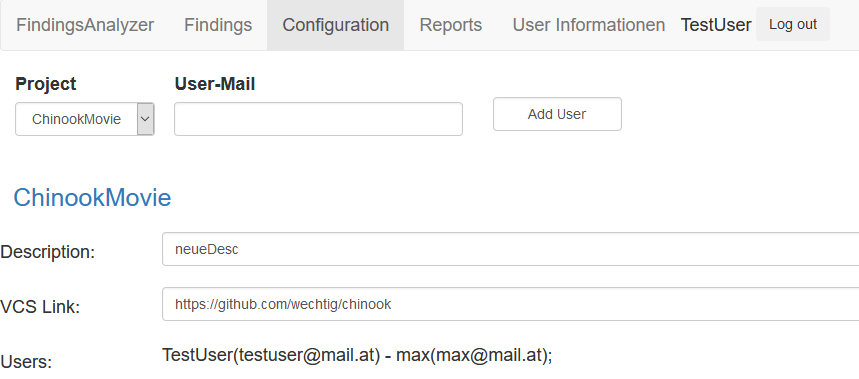
\includegraphics[height=6cm]{images/configuration.PNG}
  % The short caption should be capitalised
  % The full caption should hold a full sentence. 
 \caption[Konfiguration für das Projekt und Team]{Unterseite für verschiedene Konfigurationen für das Projekt und das Team. In diesem Beispiel ist der angemeldete User \textit{TestUser} Mitglied des Teams für das Projekt \textit{ChinookMovie}. So kann er neue Mitglieder zum Team hinzufügen.}
  \label{fig:configuration}
\end{figure}
\section{Anbindung der Versionsverwaltung für spezifische User-Unterstützung}
\subsection{Allgemeines}
Auf der Hauptseite der Webapplikation werden alle Fehler, Code Smells, Warnungen und Bugs gelistet, die die Tools der Statischen Code Analyse im Projekt finden und welche mit den Importer-Plugin in die Datenbank importiert werden. Diese Informationen werden alle in einer Tabelle angezeigt, welche nach Projekt, Klasse oder Datum sortiert und gefiltert werden kann. \\
Das Problem bei dieser Implementierung ist die unspezifische Anzeige: Den Teammitgliedern werden alle Informationen angezeigt, auch Fehler, die von anderen Entwicklerinnen oder Entwicklern implementiert worden sind. So können  Fehler im Projekt gefunden werden und das Team kann die Fehler einsehen. Das Problem bei einer dauerhaften Verbesserung der Kenntnisse der Entwicklerinnen und Entwickler ist hierbei aber die unpersönliche Anzeige. Um den Usern der Webapplikation die genauen Fehler anzuzeigen wird Lösung mit der Anbindung eines VCS-Tools (Version Control System) implementiert. Das Konzept dabei ist es, das die angemeldeten User mit den VCS-Usern verbunden werden. So können die genauen Implementierungen untersucht werden. Dabei werden zum Beispiel die committeden Klassen aus den einzelnen gelesen.
\subsubsection{Ablauf}
Um die spezifische User Unterstützung benutzen zu können, muss im Projekt eine Versionsverwaltung verwendet werden (Im Rahmen dieser Arbeit wurde hierbei die Unterstützung für die Versionsverwaltung Git implementiert). Der Link des Repositories muss zusätzlich in der Projektkonfiguration von einem Teammitglied konfiguriert werden (siehe Abbildung 4.1). Um nun die Accounts der Teammitglieder in der Userverwaltung mit den Entwicklerinnen und Entwicklern des Projekts in der Versionsverwaltung verbinden zu können, wird die Email-Adresse verwendet. Das heißt, die Email-Adresse im Tool der Versionsverwaltung muss mit der Email-Adresse der Userverwaltung übereinstimmen. Werden nun in der Weboberfläche die Informationen zu der Statischen Code Analyse abgefragt, so werden die Informationen in der Datenbank mit den Daten der Versionsverwaltungs-API verglichen und es wird versucht eine Verbindung herzustellen. Es werden nur jene Fehler und Informationen abgefragt und angezeigt, die vom angemeldeten User implementiert und committed worden sind.   
\subsubsection{Alternative Implementierungsmöglichkeiten}
Die beschriebene Methode mit der Einbeziehung eines Versionsverwaltungstools ist nur eine mögliche Methode zur persönlichen Anzeige. Ein Problem bei dieser Methode ist die verpflichtende Angabe eines VCS-Links. Andere Möglichkeiten, die diese Konfiguration nicht verlangen, sind unter anderem: \\
\textbf{Angabe der entwickelnden Klassen und Methoden} \\
Hierbei könnten die Entwicklerinnen und Entwickler die entwickelnden Methoden und Klassen in einer Übersichtsseite auswählen. Fehler, Bugs und andere Meldungen aus diesen Klassen werden den Usern angezeigt.\\
\textbf{Automatische Erkennung durch Verteilung der Aufgaben} \\
Die Idee bei dieser Methode ist eine Konfiguration, wo die Aufgaben verteilt werden: Die Benutzerinnen und Benutzer könnten hierbei jene Packages oder Module angeben, welche sie entwickeln. So können zum Beispiel die Aufgaben als Packages wie Repositories, Modules oder Weboberfläche verteilt werden. \\
\textbf{Autorennamen verwenden} \\
Bei dieser möglichen Lösung werden die Autorangaben der \textit{Javadoc} verwendet. Bei der \textit{Javadoc} zu Klassen werden unter anderem die Autoren angegeben \footnote{https://www.oracle.com/technical-resources/articles/java/javadoc-tool.html}. Dieser Autorenname kann dazu verwendet werden, um den angemeldeten Usern die richtigen Meldungen anzuzeigen, wenn die beiden Namen übereinstimmen.
\subsection{GithubAPI und Service}
Mit der GithubAPI können anderem die Commits eines Repositories abgefragt werden. Dazu müssen der User und der Name des Repositories bekannt sein. Um genauere Abfragen zu erstellen, wird auch ein Datumsbereich angegeben. Aus diesen Variablen wird ein Pfad erstellt, mit dem die Daten abgefragt werden (siehe 4.3.2.1). Der Pfad zum Repository muss in der Oberfläche für die Konfiguration angeben werden, die anderen Daten kann die Benutzerin oder der Benutzer bei der Abfrage auf der Weboberfläche auswählen. 
\subsubsection{HttpClient und API-Abfrage}
Der \textit{HttpClient} ist seit Java 11 ein Teil von Java \footnote{https://openjdk.java.net/groups/net/httpclient/intro.html}. Mit dem HttpClient können unter anderem Http-Daten abgefragt werden. Der \textit{HttpClient} wird in der Arbeit dazu verwendet, um die Daten der GithubAPI abzufragen. Dazu wird der Github-API-Pfad verwendet. Der \textit{HttpClient} benötigt zur Abfrage noch einen \textit{HttpRequest} um den Request abzuschicken und zu verarbeiten. Im \textit{HttpRequest} können Header-Variablen(User-Agent) und die Http-Methode(Bei der Github-Abfrage die Methode \textit{GET}) angegeben werden. Der Rückgabewert kann mit dem \textit{HttpResponse} bearbeitet werden (siehe Listing   \ref{lst:httprequest}).
\lstset{
  caption=[Listing für die Implementierung für die Abfrage der Github-API und Beispiel-Request.]{Listing für die Implementierung für die Abfrage der Github-API. Am Beginn des Listings wird in einem Kommentar ein Beispiel-Link für den Request angezeigt. Im Link enthalten ist der Benutzername des Users und der Datumsbereich, aus dem die Commits geladen werden sollen.}, 
  basicstyle=\small\ttfamily, 
  label=lst:httprequest, 
  %float=tbhp, % float image to top/bottom/here/page
  language=Java,
  frame=single,
  breaklines=true, % break long source code lines, and add arrow
  postbreak=\mbox{\textcolor{red}{$\hookrightarrow$}\space},
  %  basewidth={0.55em}, 
  % fontadjust}  % adjust these for more appealing appearance
}
\begin{samepage}% with samepage we keep a FLOATing listing on one page
	\begin{lstlisting}[float=tbhp]
https://api.github.com/repos/wechtig
/chinook/commits?since=2014-07-29&until=2020-07-28
...
HttpClient httpClient = HttpClient.newBuilder()
     .version(HttpClient.Version.HTTP_1_1)
     .connectTimeout(Duration.ofSeconds(20))
     .build();

public String get(String url)  {
    HttpRequest request = HttpRequest.newBuilder()
     .GET()
     .uri(URI.create(url))
     .setHeader("User-Agent", "Java 11 HttpClient Bot")
     .build();
    try {
      HttpResponse<String> response = 
      httpClient.send
      	(request, HttpResponse.BodyHandlers.ofString());
            return response.body();
	...
	\end{lstlisting}
\end{samepage}
\subsubsection{Verarbeitung des Response}
Der \textit{HttpResponse} beinhaltet neben Informationen wie den Http-Status-Code, verschiedenen Headers und anderen Variablen einen Response-Body. Dieser Body kann als JSON gelesen und verwendet werden. Die JSON-Werte werden mit Java als \textit{Map} mit zwei \textit{String} gelesen. So kann der Variablenname und der Wert gelesen werden. Da sich im Response mehrere JSON-Werte befinden, muss zusätzlich eine Liste erstellt werden. Aus dem Response können nun die Autoren und die Commit-Links ausgelesen werden. Es werden nur jene Commits in der Liste gespeichert, wo der Autor mit dem angemeldeten Benutzer übereinstimmt. Commits von anderen Entwicklerinnen oder Entwickler werden nicht gespeichert, da sie nicht in der persönlichen Fehler- und Buganzeige auftauchen sollen. Die einzelnen Änderungen können nur über die Commit-Links herausgefunden werden, daher muss ein zweiter Request abgeschickt werden. Aus dem Response des zweiten Commit-Requests lassen sich nun die geänderten Datein (filename) auslesen \ref{lst:lstresponse}. Dazu kann der \textit{ObjectMapper} verwendet werden.
\lstset{
  caption=[Auslesen der geänderten Files aus der Github-API.]{Auslesen der geänderten Files aus der Github-API. Die Links für die Commits müssen in einem eigenen Request vom Repository ausgelesen werden.}, 
  basicstyle=\small\ttfamily, 
  label=lst:lstresponse, 
  %float=tbhp, % float image to top/bottom/here/page
  language=Java,
  frame=single,
  breaklines=true, % break long source code lines, and add arrow
  postbreak=\mbox{\textcolor{red}{$\hookrightarrow$}\space},
  %  basewidth={0.55em}, 
  % fontadjust}  % adjust these for more appealing appearance
}
\begin{samepage}% with samepage we keep a FLOATing listing on one page
	\begin{lstlisting}[float=tbhp]
...
List<String> files = new ArrayList<>();
for (String commit : commitLinks) {
   String commitData = httpGithubClient.get(commit);
   if(data == null) {
       return new ArrayList<>();
   }
   try {
     Map<String, List<Object>> commitResponse = new   
      ObjectMapper().readValue(commitData, Map.class);
     List<Object> changedFiles = 
      commitResponse.get("files");

     if(changedFiles == null) {
      continue;
     }

     for(Object o : changedFiles)  {
      String filename = 
        (String) ((LinkedHashMap) o).get("filename");
      files.add(filename);
     }
...     
	\end{lstlisting}
\end{samepage}
Nachdem die geänderten Dateien ausgelesen worden sind, werden aus der Datenbank die Fehlerinformationen und Warnung für die Datei gelesen. Bei der Datenabfrage wird auch der Datumsbereich verwendet, um genauere Anzeigen zu bekommen.
\subsection{Fehlende Informationen über die geänderten Zeilen}
Ein Problem bei der Unterstützung der GithubAPI, ist die fehlende Information über die genauen geänderten Zeilen. Denn mit der GithubAPI ist es nur möglich, die geänderten Dateien auszulesen, nicht aber genaue die geänderten Zeilen. So ist es möglich, das ein anderes Teammitglied den Fehler bereits früher in die Klasse eingebaut hat. Wenn die Klasse beim Commit geändert wird, so wird auch dieser Fehler angezeigt. Wenn aber eine Entwicklerin oder ein Entwickler Änderungen an einer Klasse vorgenommen hat und Fehler übersehen oder nicht die Kenntnisse über den Fehler hat, so ist es auch ein möglicher Vorteil für das Teammitglied, wenn der Fehler in der Übersicht angezeigt wird. 
\subsection{Oberfläche}
Die Oberfläche für die persönliche Fehler und Warnungsanzeige des Users ist identisch mit der allgemeinen Übersichtsansicht. Zusätzlich wurde aber eine Github-Verlinkung für die Fehler in der Tabelle eingebaut. Dieser Link wurde auf die Anzeige der betreffenden Zeilennummer gesetzt (siehe Abbildung 4.3). Über diesen Link kann der Code in der Online-Versionsverwaltung eingesehen werden. Der Link wird hierbei aus dem Link für das Repository in der Konfiguration, aus dem Filenamen und den Zeilennummern erstellt. Dadurch, dass im Link die Zeilennummern hinzugefügt werden, kann die genaue Zeile angezeigt werden. Auch Fehler, die sich über mehrere Zeilen strecken, werden markiert (siehe Abbildung \ref{fig:markedFindings}). 
\begin{figure}[tp]
  \centering
  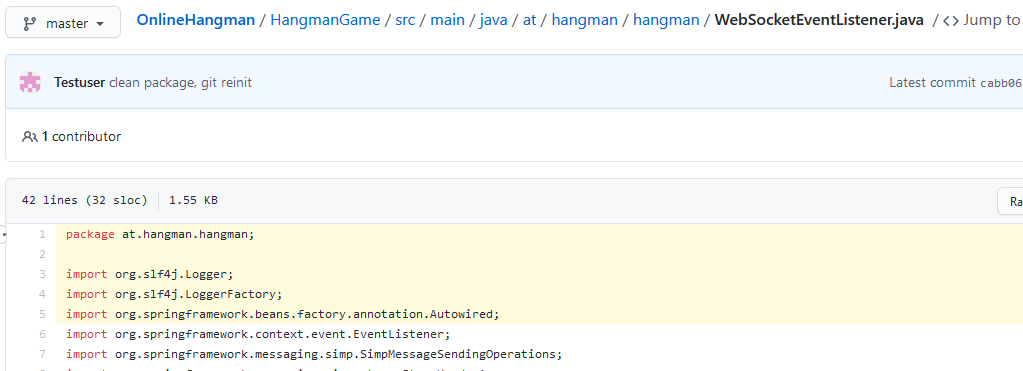
\includegraphics[height=5cm]{images/markedFindings.PNG}
  % The short caption should be capitalised
  % The full caption should hold a full sentence. 
 \caption[Anzeige der markierten Fehler]{Über einen Link kann der Fehler im Code genau markiert und angezeigt werden.}
  \label{fig:markedFindings}
\end{figure}
\section{Cron Job und Report Sender für Berichte}
\subsection{Automatische Berichte} 
Mit dem Cron Job Reporter können Teams regelmäßige Berichte vom Projekt direkt erhalten. Die Reports von einem Projekt werden direkt an alle Teammitglieder geschickt. So können die wichtigsten Informationen, Charts und Änderungen eingesehen werden, ohne dass die Webapplikation benutzt werden muss. Dieser Bericht soll regelmäßig (Einmal in der Woche) automatisch versendet werden. Dafür wird ein Cron Job verwendet. Der automatische Bericht kann unter anderen für Projektmanager oder Scrum-Master verwendet werden, welche an mehreren verschiedene Projekten beteiligt sind. Aber auch die Entwicklerinnen und Entwickler können so schnell die neuesten Änderungen einsehen. \\ Ein Cron Job bzw. ein Scheduler ist eine Implementierung, die einen bestimmten Task immer wieder zu einem bestimmten Zeitpunkt ausführt. Spring bietet die Möglichkeit, solche Scheduler zu erstellen. Dazu muss das Keyword \textit{Scheduled} zusammen mit einer Cron-Expression verwendet werden ~\parencite{cintirScheduler}. Diese Konfiguration wird bei einer Methode angewandt, welche die neuen Fehler und Warnungen der letzten Woche aus der Datenbank ausliest und daraus einen Report generiert. Ebenso werden die Charts eingebunden. Der Report wird danach mit dem Mail-Cient versendet (siehe 4.4.3). Mit einer Cron-Expression kann der Zeitpunkt festgelegt werden, wann die Berichte versendet werden sollen. Die Cron-Expression kann im File \textit{application.yml}(YAML-Framework) definiert werden, der Standardwert der Cron-Expression ist \textit{0 0 12 ? * 6}, also jeden Freitag um 12:00. Das YAML-Framwork ist ein Framework für die einfache Serealisierung von Daten, also für die Persistierung eines Objekts um Daten und Informationen zu speichern ~\parencite{eriksson2011comparison}. So können die Informationen einfach gespeichert und ausgelesen werden. In Spring kann aber zur Alternative das File \textit{application.properties} verwendet werden. \\ Um den Scheduler bei der Spring-Security verwenden zu können, muss bei den Sicherheitskonfiguration (\textit{WebSecurityConfigurerAdapter}) der Scheduler zugelassen werden. Für den Spring Scheduler können eigene XML-Konfigurationsdateien erstellt werden, in der zum Beispiel die Cron-Expression auch definiert werden kann.
\subsection{Manuelle Berichte}
Auch manuell können Berichte an bestimmte Personen verschickt werden. Für das manuelle Versenden der Berichte gibt es in der Webapplikation eine eigenen Unterseite: \textit{Reports}. Dort kann das Projekt und der Zeitraum ausgewählt werden, aus welchen der Report generiert werden soll. Der generierte Report kann an das Team oder an eine selbst gewählte Email-Adresse versendet werden. Ebenso kann auch ausgewählt werden, ob der Bericht nur die Charts beinhalten soll oder auch ein Listing der neuen Fehler und Meldungen.
\subsection{Versenden der Reports mit Java Mail}
Der PDF-Report wird aus den Daten mit iText-PDF generiert (siehe Bacherlorarbeit 1). Die Charts werden ebenso in den PDF-Report eingefügt. Erstellt werden die Charts aber mit dem JavaScript-Framework Chart.js im Frontend und sie werden nach der Generierung an den Server übermittelt. Die Charts werden am Server mit dem Informationen wie Zeitraum der Daten und Projektname gespeichert. So können die Charts bei der Generierung vom Server geladen und eingefügt werden. Die PDF-Reports werden nach der Erstellung mit dem Java-Mail Client versendet. 
\subsubsection{Implementierung und Konfiguration} 
Aus den Daten und Reports wird mit JavaMail eine \textit{MimeMessage} generiert. Bei einer \textit{MimeMessage} können Informationen wie Empfänger, Anhang, Text und Betreff angegeben werden ~\parencite{harold2013javamail}. Da eine PDF an die Mail angehängt wird, muss auch ein \textit{MimePart} angegeben werden, indem der Datentyp PDF definert wird. Um eine \textit{MimeMessage} aber erstellen zu können, wird eine Session benötigt. Die Session kann ein Mail-Server sein, über diese Session wird also die Nachricht übermittelt. Da für die Arbeit kein eigener Mail-Server zur Verfügung stand, wurde ein einfacher Mail-Account angegeben. Die Mails werden dann über diesen Mail-Account gesendet. Für den Mail-Account muss eine Email-Adresse und das Passwort angegeben werden. Viele Mail-Programme blockieren aber initial eine solche Versendung der Mails, dies kann aber aktiviert werden. Nachdem die Session erstellt wurde, müssen noch Einstellung wie SMTP-Host, Port und andere Informationen angegeben werden. SMTP ist das Protokoll das verwendet werden muss, um die Emails versenden zu können. Als SMTP-Host wurde also bei der Arbeit der Gmail-Host verwendet (smtp.gmail.com). Der Gmail-Host kann aber nur verwendet werden, wenn gewisse Security-Einstellungen am Email-Account vorgenommen werden.Beim Einsatz der Applikation, beispielsweise in einem Unternehmen, kann der SMTP-Server durch einen eigenen internen SMTP-Server ersetzt werden.
\section{Kommentare}
Die Kommentare, die zu den einzelnen Meldungen erfasst werden können, sollen die Interaktion der Teammitglieder vereinfachen.
\subsection{Allgemeines und Vergleich zu Pull Requests}
\begin{figure}[tp]
  \centering
  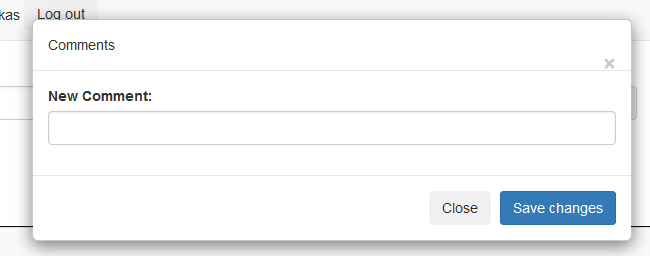
\includegraphics[height=5cm]{images/popup.PNG}
  % The short caption should be capitalised
  % The full caption should hold a full sentence. 
 \caption[Popup für das Speichern von Kommentaren]{Popup für das Speichern von Kommentaren. Beim Popup für das Anzeigen von Kommentaren wird das Eingabefeld durch ein Listing der Kommentare ersetzt.}
  \label{fig:table}
\end{figure}
Ein wichtiger Teil des Git-Workflows um Code Qualität sicher zustellen, sind die sogenannten \textit{Pull Requests} (siehe Kapitel 2.3). Pull Requests werden dazu verwendet, um neuen Code von einem bestimmten Branch (Zweig) in die gemeinsame Codebasis zu integrieren. Die Integration von fehlerhaften Code oder von Code mit schlechter Qualität soll vermieden werden. Bei Pull Requests werden daher Kommentare und Anmerkungen von anderen Teammitgliedern zu neuen Code erstellt. Werden Fehler oder Probleme bei Pull Request vom Reviewer festgestellt, bessert diese die Entwicklerin oder der Entwickler aus. \\ Mit der Kommentarfunktion können in der Weboberfläche die verschiedenen Meldungen von allen Teammitgliedern in der Übersichtstabelle kommentiert und angezeigt werden (siehe Abbildung \ref{fig:table}). Diese Kommentare unterscheiden sich von den Kommentaren in Pull Requests daher, dass sie Informationen für alle Entwicklerinnen und Entwickler darstellen. So können Kommentare, die Verbesserungsvorschläge oder andere hilfreiche Informationen beinhalten, den ganzen Team helfen. Ebenso werden diese Kommentare dauerhaft gespeichert und angezeigt werden, während Pull Requests gelöscht werden. Die Kommentare beziehen sich auch inhaltlich auf den Fehler und sollen Verbesserungsvorschläge beinhalten, während Kommentare in Pull Requests meist nur auf Fehler hinweisen. Bei der persönlichen Fehleranzeige können daher auch keine Kommentare hinzugefügt und angezeigt werden.
\subsection{Implementierung}
Um ein Kommentar speichern zu können, muss in der Übersichtstabelle das Kommentar-Popup geöffnet werden. In diesem Bootstrap-Popup kann das Kommentar eingegeben und gespeichert werden. Die Kommentare werden in einer eigenen Collection \textit{comments} gespeichert. Über einen eigenen Button können die Kommentare angezeigt werden (siehe Abbildung \ref{fig:popup}). Die Kommentare werden hierbei in das Popup geladen. \\ Wird der Datenbankimport wiederholt ausgeführ, um Informationen über einen längeren Zeitraum zu erhalten, so wird der selbe Fehler öfters in der Datenbank gespeichert.
\begin{figure}[tp]
  \centering
  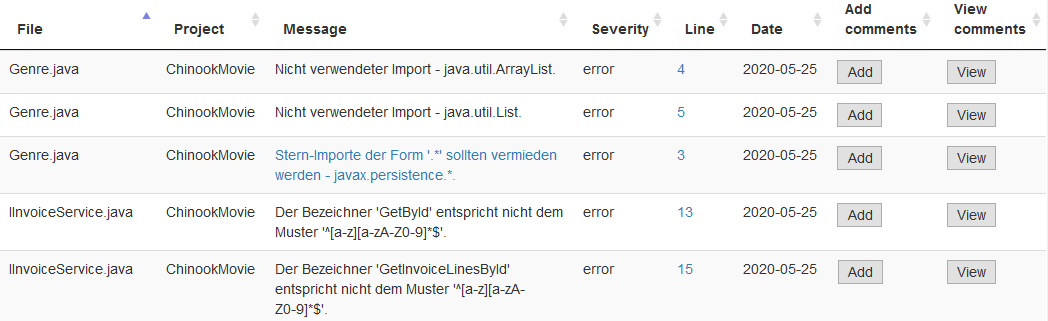
\includegraphics[height=5cm]{images/table.PNG}
  % The short caption should be capitalised
  % The full caption should hold a full sentence. 
 \caption[Übersichtstabelle]{Übersichtstabelle mit der Auflistung der Meldungen. Mit den zwei Buttons können die Kommentare erstellt und angezeigt werden. Die Zeilennummer ist ein Link für die Öffnung und Anzeige des Fehlers und des Codes in der Versionsverwaltung Github. Der Link kann nur erstellt werden, wenn in der Konfiguration das Repository angegeben ist. Die Tabelle wurde mit Pagination erstellt: So kann in der Tabelle navigiert werden, sodass nie die ganze Tabelle angezeigt wird. }
  \label{fig:popup}
\end{figure}
Ein Kommentar, das daher zu einer bestimmten Meldung erfasst wird, soll aber auch für die selben anderen Meldungen gelten, welche bei wiederholten Importen gespeichert werden. Daher wird beim Auslesen der Kommentare aus der Datenbank nicht eine bestimmte Identifikationsnummer benutzt, sondern die Attribute die das Kommentar bestimmen (Projekt, Klasse, Meldung, Zeile). So wird bei allen gleichen Meldungen der Kommentar angezeigt.
\section{Android Applikation}
\subsection{Allgemeines und Idee}
Die Android Applikation soll eine neue Möglichkeit sein, um die Code Qualität zu steigern. Die wichtigsten Informationen aus der Webapplikation sollen hierbei kompakt angezeigt werden: Die einzelnen Meldungen und die verschiedenen Charts. Die Möglichkeit zur Filterung nach Projekt und Zeitbereich soll auch hierbei verfügbar sein. Die Applikation wurde mit Java entwickelt. \\ Die Applikation verwendet keinen direkten Zugriff auf die Datenbank. So konnte unter anderem doppelter Code vermieden werden, da Services und Repositorys nicht für beiden Applikationen entwickelt werden . Die mobile Applikation bezieht die Daten aus der API der Webapplikation. Dazu werden mit verschieden Attributen HTTP-Requests abgeschickt. Die HTTP-Parameter die benötigt werden um die Daten aus der Datenbank abzufragen, kann die Benutzerin oder Benutzer beim Start der Applikation auswählen. Die Webapplikation wiederum liest die Daten mithilfe der Services und des MongoDB Java Drivers aus der Datenbank aus. Der Aufbau der Applikation beinhaltet Java-Packages für die Datenhaltungsklassen und die Business-Logik wie HTTP-Tasks, sowie auch die Aktivitäten (siehe Abbildung 4.5).

\begin{figure}[tp]
  \centering
  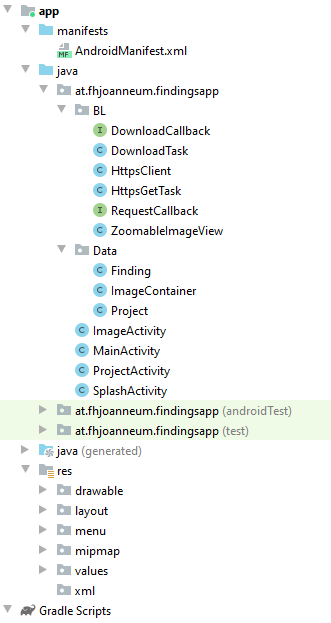
\includegraphics[height=8cm]{images/androidPackages.PNG}
  % The short caption should be capitalised
  % The full caption should hold a full sentence. 
 \caption[Aufbau und package-Struktur der Webapplikation]{Aufbau und package-Struktur der Webapplikation. Im package \textit{manifests} wird das Android-Manifest definiert. Die Datenhaltungsklassen, Aktivitäten und die Business-Logic befinden sich im Package \textit{java}. Im Folder \textit{res} befinden sich die Inhalte zum Layout der Applikation.}
  \label{fig:popup}
\end{figure}


\subsubsection{Neuer Funktion zur Steigerung der Kenntnisse}
In der Applikation soll ebenso ein neuer Aspekt oder eine neue Funktion implementiert werden, die der Unterstützung der Kenntnisse über bestimmte Fehler dient. Implementiert wurde so eine kleine spielerische Funktion, mit der die Entwicklerinnen und Entwickler unterstützt werden sollen. Diese Funktion wurde als Shake-Funktion entwickelt, mit der zufällige Inhalte angezeigt werden. Wird also das mobile Gerät geschüttelt, so werden zufällige Meldungen oder Charts angezeigt.
\subsection{Abfrage der Daten}
Um die Informationen verwendet zu können, wird ein Request verwendet. Der Request wird als HTTP-Get-Funktion implementiert. Mit den Informationen zu Projekt und Datumsbereich wird die URL erstellt. Mit einer \textit{HttpURLConnection} wird der Request abgeschickt ~\parencite{liu2017web}. Auch andere Http-Funktionen werden von der Klasse \textit{HttpURLConnection} unterstützt, daher muss die HTTP-Methode \textit{Get} aber auch andere Optionen wie das \textit{Timeout} angegeben werden. Der Request wird daraufhin vom Controller in der Webapplikation verarbeitet und eine Response enthält die Charts und Informationen. Ist der Response-Code der Wert 200 (OK), so wird der Response mit einem \textit{BufferedReader} und einem \textit{InputSream} gelesen. Die Daten werden an die Aktivität als JSON-Wert zurückgegeben. Um die Daten aus dem JSON-Result verwenden zu können wurde noch ein \textit{JSONArray} benutzt, von dem die verschiedenen \textit{JSONObjects} ausgelesen und zu Java-Objekten umgewandelt wurden. 
\subsection{Aktivitäten und Navigation}
Eine \textit{Activity} wird für einen bestimmte Anzeige, also zum Beispiel ein Formular oder ein Bildschirm, erstellt ~\parencite{mednieks2012programming}. Diese Aktivitäten werden im Android Manifest registriert. Ebenso kann zu den Aktivitäten eine Layout-Klasse erstellt werden. Diese Layout-Klasse wird in der \textit{Activity} registriert. Zwischen den einzelnen Aktivitäten soll der Benutzer wechseln können, entweder manuell oder automatisch. In der Applikation gibt es vier Aktivitäten (siehe Abbildung 4.6):
\begin{figure}[tp]
  \centering
  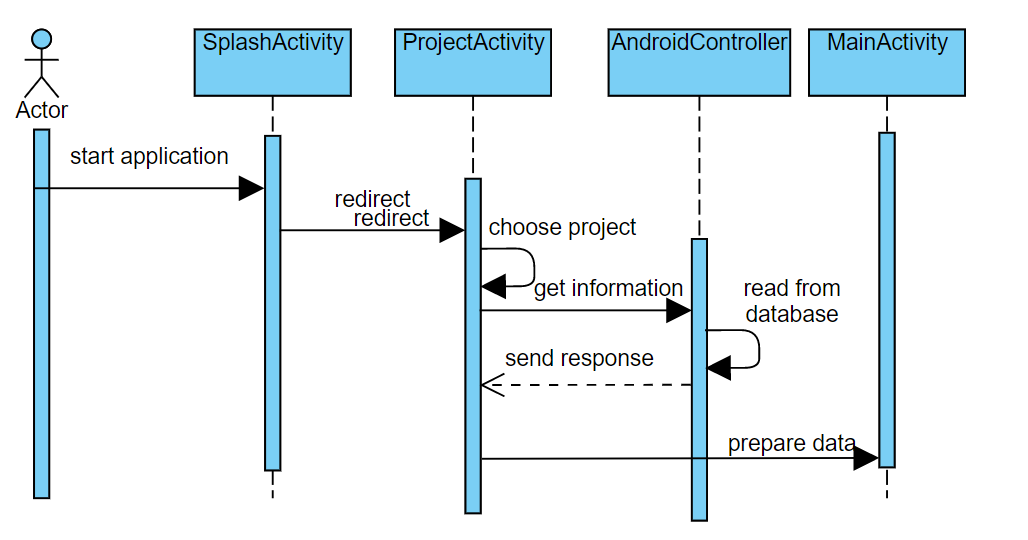
\includegraphics[height=8cm]{images/seqAct.PNG}
  % The short caption should be capitalised
  % The full caption should hold a full sentence. 
 \caption[Sequenzdiagramm für die Interaktion der verschiedenen Activities untereinander und mit der Webapplikation.]{Sequenzdiagramm für die Interaktion der verschiedenen Activities untereinander und mit der Webapplikation (Controller).}
  \label{fig:popup}
\end{figure}
\subsubsection{SplashActivity}
Die SplashActivity wird zuerst initial ausgeführt. Dies kann im Android-Manifest mit der Option \textit{android.intent.category.LAUNCHER} festgelegt werden. Während des Startvorgangs wird ein \textit{SplashScreen} kurz angezeigt. Der Benutzer wird danach automatisch zur nächsten Aktivität weitergeleitet. Dieser Startbildschirm dient zur Information und zum Erstellen der Applikation und andere Ladevorgänge. \\ Während des \textit{SplashScreen} wird der erste Request erstellt: Hierbei werden von der Webapplikation die Projektdaten geladen. Mittels eines Intents wird die nächste Aktivität \textit{ProjectActivity} danach automatisch gestartet und die Projektdaten werden weitergegeben. Ein Intent ist eine klare Funktion oder Aufgabe in der Android-Applikation, zum Beispiel der Start einer anderen Aktivität ~\parencite{vogelIntent}.
\lstset{
  caption=[Starten einer neuen Aktivität.]{Listing für die Erstellung eines neuen Intents, für den Wechsel der \textit{Activity} zur \textit{ProjectActivity}. Im Intent werden die geladenen Projektnamen hinzugefügt und in der neuen \textit{Activity} ausgelesen.},
  basicstyle=\small\ttfamily, 
  label=lst:config, 
  %float=tbhp, % float image to top/bottom/here/page
  language=Java,
  frame=single,
  breaklines=true, % break long source code lines, and add arrow
  postbreak=\mbox{\textcolor{red}{$\hookrightarrow$}\space},
  %  basewidth={0.55em}, 
  % fontadjust}  % adjust these for more appealing appearance
}

% listing with some settings, such as float, for this listing only
\begin{samepage}% with samepage we keep a FLOATing listing on one page
	\begin{lstlisting}[float=tbhp]
...
Intent intent = new Intent
   (SplashActivity.this, ProjectActivity.class);
ArrayList<String> projects = 
   new ArrayList<>(Arrays.asList(projectsArray));
intent.putStringArrayListExtra("Projects", projects);
startActivity(intent);
...  

	\end{lstlisting}
\end{samepage}
\subsubsection{ProjectActivity}
In der \textit{ProjectActivity} werden die Projektdaten aus dem Intent ausgelesen. Die Projektnamen werden im dazugehörigen Layout in einer \textit{SelectBox} angezeigt. Ebenso gibt es im Projekt-Layout zwei Date-Picker, mit dem der Datumsbereich der Abfrage festgelegt werden kann. Nachdem die Benutzerin oder der Benutzer einen Datumsbereich und ein Projekt ausgewählt hat, wird die eingegebenen Daten in der Aktivität gespeichert. Nachdem die Benutzerin oder der Benutzer alle Daten eingegeben hat, wird automatisch die nächste Aktivität aufgerufen. Die ausgewählten Parameter Projektname und Datumsbereich werden wieder in einem Intent gespeichert und die nächste Aktivität wird automatisch aufgerufen.
\begin{figure}[tp]
  \centering
  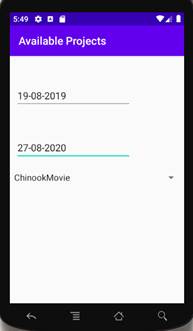
\includegraphics[height=8cm]{images/anroidProjectScreen.PNG}
  % The short caption should be capitalised
  % The full caption should hold a full sentence. 
 \caption[Layout für die Auswahl des Zeitbereichs und des Projekts]{Layout für die Auswahl des Zeitbereichs und des Projekts. Die Datumswerte werden über einen DatePicker eingegeben. Sobald alle Informationen eingegeben worden sind, wird die nächste \textit{Activity} aufgerufen.}
  \label{fig:findingsInIDE}
\end{figure}
\subsubsection{MainActivity}
Die \textit{MainActivity} ist die zentrale Aktivität der Applikation. Im Layout zur \textit{MainActivity} werden die Meldungen, Bugs und Fehler angezeigt. \\ Bevor die Aktivität angezeigt wird, werden die Parameter aus dem Intent gelesen. Mit diesen Parametern wird ein Request durchgeführt und die Meldungen werden im Backend der Webapplikation aus der Datenbank ausgelesen und zurückgegeben. Der Response wird in der mobilen Applikation zu einer Liste von Meldungen konvertiert. Aufgrund der Größe des Textes der Fehlermeldungen werden die Informationen nicht in einer gemeinsamen Liste oder auf einen Bildschirm angezeigt, sondern einzeln. Durch zwei Buttons im Footer kann die Benutzerin oder der Benutzer  nach vor oder zurück in der Liste navigieren und die Fehler genau einsehen. Dabei wird auch die Klasse und die Zeilennummer der Meldung angezeigt. Wird das mobile Geräte bei dieser Aktivität geschüttelt, so wird eine zufällige Meldung angezeigt (siehe Punkt 4.6.4). Ebenso gibt es im Footer ein Image-Icon, das die Möglichkeit bereitstellt, die generierten Charts, erstellt aus den Meldungen, anzuzeigen (siehe Bac 2 TODO). Wird diese Option ausgewählt, wird die Aktivität gewechselt, und die \textit{ImageActivity} aufgerufen.
\begin{figure}[tp]
  \centering
  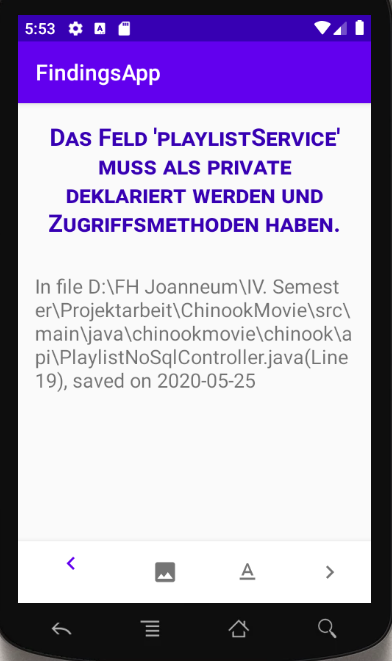
\includegraphics[height=8cm]{images/androidFindingScreen.PNG}
  % The short caption should be capitalised
  % The full caption should hold a full sentence. 
 \caption[Layout für die Anzeige der Meldungen.]{Layout für die Anzeige der Meldungen.}
  \label{fig:findingsInIDE}
\end{figure}
\subsubsection{ImageActivity}
In der \textit{ImageActivity} werden die Parameter zunächst wieder ausgelesen. Mit den Parametern wird ein Request geschickt und die Charts von der Webapplikation geladen. Die Bilder werden in einer \textit{ImageView} im Layout angezeigt (siehe Abbildung 4.7). Auch hierbei besteht wieder die Möglichkeit zwischen den Bildern zu navigieren. Ebenso wird auch ein zufälliges Charts angezeigt, wenn das mobile Gerät geschüttelt wird. Im Footer des Layouts zur \textit{ImageActivity} gibt es wieder die Option, zur \textit{MainActivity} zu wechseln. Die Charts können in der Oberfläche auf vergrößert werden, um Details einsehen zu können.  \\
\textbf{Fehlende Generierung der Charts am Backend} \\
Ein Problem bei dieser Lösung ist, das die Charts nicht im Backend der Webapplikation oder in der Android-Applikation generiert werden können (siehe Punkt 4.4.3). Daher können nur jene Charts von der mobilen Applikation angezeigt werden, welche bereits in der Webapplikation vom Frontend generiert worden sind. Eine Lösung, die dieses Problem beheben könnte, ist die Verwendung einer anderen Art der Erstellung und Speicherung der Charts. So könnten diese zum Beispiel mit einer Library wie der \textit{Google Chart API}\footnote{https://developers.google.com/chart/?csw=1} oder \textit{JFreeChart}\footnote{http://www.jfree.org/jfreechart/} am Backend generiert, gespeichert und nach Bedarf an die Android-Applikation übermittelt werden.
\begin{figure}[tp]
  \centering
  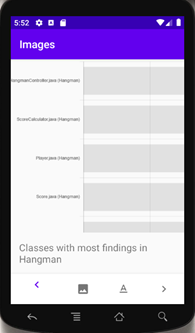
\includegraphics[height=8cm]{images/androidChart.PNG}
  % The short caption should be capitalised
  % The full caption should hold a full sentence. 
 \caption[Layout für die Anzeige der generierten Charts]{.Layout für die Anzeige der generierten Charts}
  \label{fig:findingsInIDE}
\end{figure}
\subsection{Shake-Funktion}
Mit der Shake-Funktion soll ein neuer spielerischer Aspekt in die Applikation eingebaut werden. Diese Funktion soll Benutzerinnen und Benutzer, die Verwendung der Applikation vereinfachen und die Erfahrung verbessern. Aber auch andere spielerische Funktionen können noch in die Applikation eingebaut werden (siehe Punkt 6). \\
Mit der Shake-Funktion sollen zufällige Meldungen und Charts beim Schütteln der Applikation angezeigt werden. Dies funktioniert mit einem eigenen Sensor ~\parencite{borckanalyse}: Der \textit{SensorEventListener } kann dazu verwendet, um herauszufinden ob sich das mobile Gerät bewegt hat. Wird das Gerät bewegt, wird ein \textit{SensorEvent} ausgelöst \footnote{https://developer.android.com/reference/android/hardware/SensorEvent}. 
\lstset{
  caption=[Listing für die Implementierung des SensorEventListener.]{Listing für die Implementierung des SensorEventListener. Reagiert der Sensor auf eine Bewegung, wird das Event ausgelöst. Mit der Berechnung der \textit{Acceleration} wird festgestellt, ob sich das mobile Gerät schnell genug bewegt hat und so ob die Shake-Funktion bewusst ausgeführt werden soll. Sonst würde das Event auch bei kleinsten Bewegungen reagieren. Ist die Beschleunigung schnell genug, so wird eine zufällige Meldung geladen.},
  basicstyle=\small\ttfamily, 
  label=lst:config, 
  %float=tbhp, % float image to top/bottom/here/page
  language=Java,
  frame=single,
  breaklines=true, % break long source code lines, and add arrow
  postbreak=\mbox{\textcolor{red}{$\hookrightarrow$}\space},
  %  basewidth={0.55em}, 
  % fontadjust}  % adjust these for more appealing appearance
}

% listing with some settings, such as float, for this listing only
\begin{samepage}% with samepage we keep a FLOATing listing on one page
	\begin{lstlisting}[float=tbhp]
...
private final SensorEventListener 
    sensorListener = new SensorEventListener() {
     @Override
     public void onSensorChanged(SensorEvent event) {
       float x = event.values[0];
       float y = event.values[1];
       float z = event.values[2];
       lastAcceleration = currentAcceleration;
       currentAcceleration = 
            (float) Math.sqrt((x * x + y * y + z * z));
       float delta = currentAcceleration - lastAcceleration;
       acceleration = acceleration * 0.9f + delta;
       if (acceleration > 12) {
            getRandomFinding();
       }
     }
...  .passwordEncoder(bCryptPasswordEncoder);
}
	\end{lstlisting}
\end{samepage}

In diesem Kapitel wurde die verschiedenen neuen Aspekte und Funktionen beschrieben und die dazugehörige Implementierungen. Im folgenden Kapital \textit{Evaluierung} wird die Implementierung interpretiert und die Ergebnisse werden ausgearbeitet.

\chapterend